\chapter{Konduktor dan Isolator}\label{ch:g4:conductors-insulators}

Mengapa kawat listrik dibuat dari logam --- tetapi berbaju plastik?
Mengapa jembatan kecil pada \omterm{ex:g3:first-electric-circuit:switch}{sakelar} menghantarkan arus, sementara
selubungnya menjaga jarimu tetap aman? Tahun lalu kita menutup
lingkar; tahun ini kita bertanya bahan apa saja yang sanggup dilewati
listrik. Jawabannya memilah setiap bahan menjadi dua macam: \omterm{def:g4:conductors-insulators:conductor}{konduktor}
dan \omterm{def:g4:conductors-insulators:insulator}{isolator}.

\section{Alat penguji}

\begin{method}[Membuat alat penguji]\label{met:g4:conductors-insulators:tester}
Bangunlah lingkar tahun lalu --- \omterm{def:g3:first-electric-circuit:battery}{baterai}, kawat, \omterm{def:g3:first-electric-circuit:bulb}{bohlam} --- tetapi
sisakan satu celah yang disengaja: dua ujung kawat bebas, terpisah
selebar jari.
\begin{enumerate}
  \item sentuhkan kedua ujung bebasnya: \omterm{def:g3:first-electric-circuit:bulb}{bohlamnya} menyala ---
        alat pengujinya bekerja;
  \item jembatani celahnya dengan benda yang diuji, satu ujung
        logamnya ditekan erat pada tiap kawat;
  \item amati \omterm{def:g3:first-electric-circuit:bulb}{bohlamnya}: menyala berarti listrik menyeberangi
        bendanya; gelap berarti listrik tidak dapat menyeberang.
\end{enumerate}
\omterm{def:g3:first-electric-circuit:bulb}{Bohlamnya} yang memberi jawaban: ia menyala tepat ketika benda yang
diuji melengkapi lingkarnya.
\end{method}

\begin{omfigure}
\begin{tikzpicture}[scale=0.9]
  \draw (0,0) to[battery1, l=baterai] (0,2.6)
    to[short] (2.2,2.6)
    to[lamp, l=bohlam] (4.4,2.6)
    to[short] (6.0,2.6) -- (6.0,1.7);
  \draw (6.0,0.9) -- (6.0,0) to[short] (0,0);
  \fill (6.0,1.7) circle (1.6pt) node[right, font=\small]
    {~ujung bebas};
  \fill (6.0,0.9) circle (1.6pt) node[right, font=\small]
    {~ujung bebas};
  \draw[thick, fill=omMeth, fill opacity=0.4]
    (5.75,0.95) rectangle (6.25,1.65);
  \node[right, font=\small] at (6.6,1.3) {benda yang diuji};
\end{tikzpicture}

{\small Alat penguji: lingkar yang sehat dengan satu celah. Apa pun
yang menjembatani celahnya sedang diuji --- \omterm{def:g3:first-electric-circuit:bulb}{bohlamnya} menunjukkan
apakah arus menyeberanginya.}
\end{omfigure}

\section{Konduktor dan isolator}

\begin{definition}[Konduktor]\label{def:g4:conductors-insulators:conductor}
Sebuah \emph{konduktor}\index{konduktor} adalah bahan yang
memperbolehkan listrik merambat melewatinya. Pada alat penguji,
konduktor yang menjembatani celahnya menutup lingkar dan menyalakan
\omterm{def:g3:first-electric-circuit:bulb}{bohlamnya}.
\end{definition}

\begin{definition}[Isolator]\label{def:g4:conductors-insulators:insulator}
Sebuah \emph{isolator}\index{isolator} adalah bahan yang menghalangi
listrik. Menjembatani celahnya dengan isolator membuat lingkarnya
tetap terbuka seperti sebelumnya: \omterm{def:g3:first-electric-circuit:bulb}{bohlamnya} tetap gelap.
\end{definition}

\begin{example}[Sepagi penuh pengujian]\label{ex:g4:conductors-insulators:trials}
Hasil dari alat penguji di ruang kelas: penjepit kertas baja ---
menyala. Sekeping koin --- menyala. Aluminium dapur --- menyala.
Sebuah kunci --- menyala. Penggaris plastik --- gelap. Pensil kayu ---
gelap. Kelereng kaca --- gelap. Penghapus karet --- gelap. Sepotong
kertas --- gelap. Polanya langsung terlihat: benda yang menyalakan
\omterm{def:g3:first-electric-circuit:bulb}{bohlam} semuanya terbuat dari logam.
\end{example}

\begin{proposition}[Logam menghantarkan]\label{prop:g4:conductors-insulators:metals}
Semua logam menghantarkan listrik --- besi, tembaga, aluminium, emas,
semuanya, itulah sebabnya kecerewetan \omterm{def:g1:magnets:magnet}{magnet} terhadap besi dahulu
mengejutkan kita tetapi alat penguji tidak akan pernah begitu.
Kebanyakan \omterm{def:g3:solids-liquids-gases:solid}{zat padat} sehari-hari yang lain --- plastik, kayu, kaca,
karet, kertas, lilin --- adalah \omterm{def:g4:conductors-insulators:insulator}{isolator}.
\end{proposition}

\begin{remark}[Konduktor bukan berarti magnetis]\label{rem:g4:conductors-insulators:notmagnet}
Jangan mencampuradukkan kedua bakat logam itu. \omterm{def:g1:magnets:magnet}{Magnet} hanya memilih
besi dan keluarganya; arus listrik jauh lebih tidak pemilih dan
merambat melewati \emph{setiap} logam. Aluminium dapur yang
mengabaikan magnetmu menghantarkan arus dengan sangat baik --- dua
permainan yang berbeda, dua aturan yang berbeda.
\end{remark}

\section{Konduktor dan isolator bekerja bersama}

\begin{example}[Anatomi sebuah kabel]\label{ex:g4:conductors-insulators:wire}
Amati ujung kabel sebuah lampu di tempat ia masuk ke steker: di dalam
membentang tembaga yang berkilau --- \omterm{def:g4:conductors-insulators:conductor}{konduktor}, jalan bagi arusnya; di
sekelilingnya membalut plastik berwarna --- \omterm{def:g4:conductors-insulators:insulator}{isolator}, pagar jalan itu.
Tembaganya yang bekerja; plastiknya menjaga arus tetap di dalam dan
jarimu tetap di luar. Setiap kabel di rumahmu memasangkan keduanya:
\omterm{def:g4:conductors-insulators:conductor}{konduktor} di dalam \omterm{def:g4:conductors-insulators:insulator}{isolator}.
\end{example}

\begin{omfigure}
\begin{tikzpicture}[scale=0.85]
  \draw[thick, fill=omExo, fill opacity=0.25]
    (0.5,0.35) rectangle (6.5,1.65);
  \draw[thick, fill=omThm, fill opacity=0.45]
    (0.5,0.78) rectangle (7.6,1.22);
  \node[right, font=\small] at (8.35,1.8) {selubung plastik: isolator};
  \draw[-Stealth, omExo] (8.3,1.8) -- (6.3,1.55);
  \node[right, font=\small] at (8.35,1.0) {inti tembaga: konduktor};
  \draw[-Stealth, omExo] (8.3,1.0) -- (7.72,1.0);
\end{tikzpicture}

{\small Sebuah kabel listrik yang ditelanjangi: jalan tembaga bagi
arusnya, di dalam pagar plastik demi keamanan.}
\end{omfigure}

\begin{omfigure}
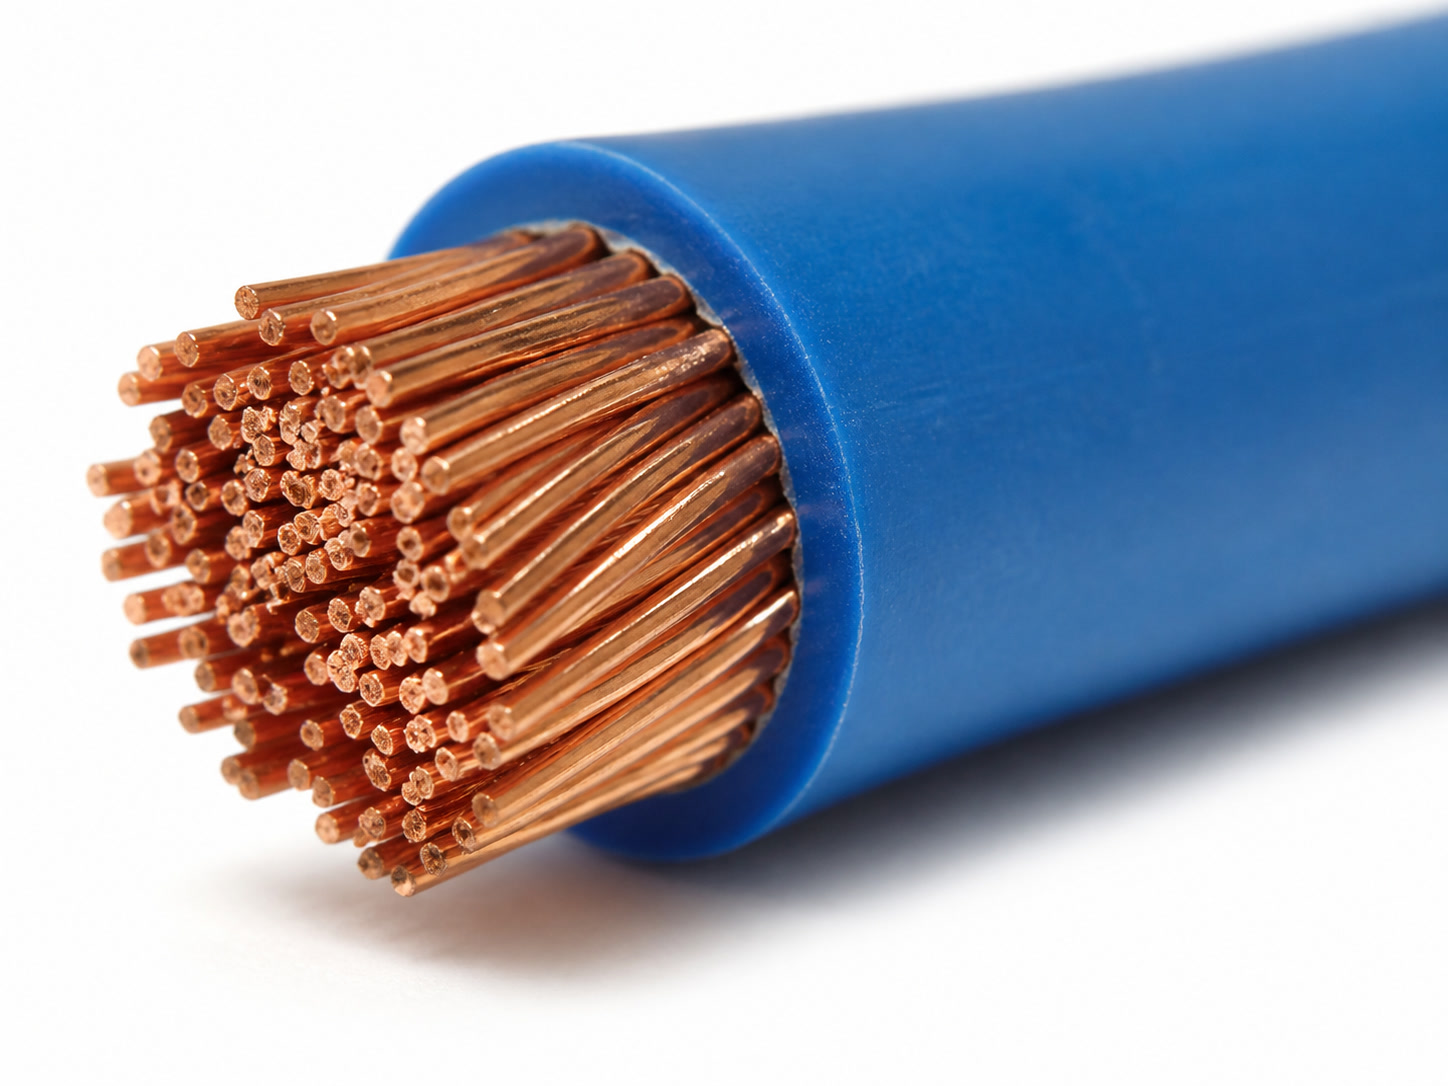
\includegraphics[width=0.5\linewidth]{images/book1/ai/g4-conductors-cable.jpg}

{\small Ujung kabel yang terpotong, sungguhan: untaian tembaga berkilau --- \omterm{def:g4:conductors-insulators:conductor}{konduktornya} --- di dalam selubung plastik berwarna --- \omterm{def:g4:conductors-insulators:insulator}{isolatornya}.}
\end{omfigure}

\begin{example}[Membaca benda sehari-hari]\label{ex:g4:conductors-insulators:objects}
Kini banyak rancangan menjelaskan dirinya sendiri. \omterm{ex:g3:first-electric-circuit:switch}{Sakelar}: jembatan
logam (ia harus membawa arus) di dalam selubung plastik (jarimu tidak
boleh). Obeng tukang listrik: bilah baja, gagang tebal yang
mengisolasi. Stopkontak: logam jauh di dalam, plastik di permukaan
luar. Menara listrik membawa kabel logam telanjang tinggi di luar
jangkauan, tergantung pada cakram pengisolasi yang panjang supaya
arusnya tidak bocor ke menaranya.
\end{example}

\begin{remark}[Air, manusia, dan mengapa ada aturan]\label{rem:g4:conductors-insulators:safety}
Satu \omterm{def:g4:conductors-insulators:conductor}{konduktor} lagi harus disebut: \emph{benda yang lembap} ---
termasuk kulit manusia yang lembap. Kita menghantarkan dengan buruk,
tetapi stopkontak mendorong begitu perkasa sehingga ``buruk'' pun
lebih dari cukup. Inilah alasan terdalam di balik aturan keselamatan
yang sudah kamu kenal: jangan pernah menyodok stopkontak, jangan
pernah menyentuh benda listrik dengan tangan basah, jauhkan pengering
rambut dari bak mandi. Alat penguji \omterm{def:g3:first-electric-circuit:battery}{baterai} aman \emph{justru karena}
dorongan \omterm{def:g3:first-electric-circuit:battery}{baterai} mungil; stopkontak tidak memaafkan apa pun.
\end{remark}

\section{Latihan}

\begin{exercise}[$\star$]\label{exo:g4:conductors-insulators:1}
Apa itu \omterm{def:g4:conductors-insulators:conductor}{konduktor}? Apa itu \omterm{def:g4:conductors-insulators:insulator}{isolator}? Yang mana yang menyalakan \omterm{def:g3:first-electric-circuit:bulb}{bohlam}
alat penguji?
\end{exercise}

\begin{exercise}[$\star$]\label{exo:g4:conductors-insulators:2}
Pilahlah menjadi \omterm{def:g4:conductors-insulators:conductor}{konduktor} dan \omterm{def:g4:conductors-insulators:insulator}{isolator}: sendok baja; \ gabus; \ aluminium dapur; \
gelas kaca; \ koin tembaga; \ balok plastik.
\end{exercise}

\begin{exercise}[$\star$]\label{exo:g4:conductors-insulators:3}
Sebelum pengujian apa pun, bagaimana kamu memeriksa bahwa alat
pengujinya sendiri bekerja? Mengapa pemeriksaan ini penting?
\end{exercise}

\begin{exercise}[$\star$]\label{exo:g4:conductors-insulators:4}
Sebuah benda uji membuat \omterm{def:g3:first-electric-circuit:bulb}{bohlamnya} tetap gelap. Berikan dua
kemungkinan sebabnya --- satu tentang bendanya, satu tentang pengujian
yang ceroboh.
\end{exercise}

\begin{exercise}[$\star$]\label{exo:g4:conductors-insulators:5}
Mengapa kabel lampu bertembaga di bagian dalam dan berplastik di
bagian luar? Apa tugas masing-masing bahan itu?
\end{exercise}

\begin{exercise}[$\star$]\label{exo:g4:conductors-insulators:6}
Pada sebuah \omterm{ex:g3:first-electric-circuit:switch}{sakelar}, bagian mana yang \omterm{def:g4:conductors-insulators:conductor}{konduktor} dan bagian mana yang
\omterm{def:g4:conductors-insulators:insulator}{isolator}? Mengapa \omterm{ex:g3:first-electric-circuit:switch}{sakelar} memerlukan keduanya?
\end{exercise}

\begin{exercise}[$\star$]\label{exo:g4:conductors-insulators:7}
Aluminium dapur sama sekali mengabaikan \omterm{def:g1:magnets:magnet}{magnet}. Apakah ia akan
menyalakan \omterm{def:g3:first-electric-circuit:bulb}{bohlam} alat penguji? Aturan mana yang menjawab, dan
kekeliruan apa yang diperingatkan oleh
\cref{rem:g4:conductors-insulators:notmagnet}?
\end{exercise}

\begin{exercise}[$\star$]\label{exo:g4:conductors-insulators:8}
Sebuah pensil adalah kayu dengan isi grafit. Alat penguji Nino tetap
gelap pada kayunya yang bercat tetapi menyala samar dari ujung ke
ujung lewat grafit yang diraut. Apa yang ditemukan Nino tentang kedua
bahan pensil itu?
\end{exercise}

\begin{exercise}[$\star$]\label{exo:g4:conductors-insulators:9}
Mengapa obeng dan tang tukang listrik bergagang plastik yang tebal?
Bahan yang mana melindungi siapa?
\end{exercise}

\begin{exercise}[$\star\star$]\label{exo:g4:conductors-insulators:10}
Sebuah rantai kalung memberi hasil ``menyala'' pada alat penguji;
kalung manik-manik kayu memberi ``gelap''; kalung manik logam yang
disimpul pada tali katun yang tebal juga memberi ``gelap'' --- padahal
setiap maniknya menghantarkan! Jelaskan hasil ketiga itu dengan
menelusuri jalan arusnya dari manik ke manik.
\end{exercise}

\begin{exercise}[$\star\star$]\label{exo:g4:conductors-insulators:11}
Mengapa jauh lebih berbahaya menyentuh benda listrik dengan tangan
basah daripada dengan tangan kering? Dan mengapa alat penguji \omterm{def:g3:first-electric-circuit:battery}{baterai}
aman untuk percobaanmu sementara stopkontak tidak pernah aman?
Pakailah \cref{rem:g4:conductors-insulators:safety}.
\end{exercise}
